\documentclass[border=10pt]{standalone}
\usepackage{fontspec}\usepackage{tikz}
\usetikzlibrary{arrows.meta,positioning}
\definecolor{NouOrange}{HTML}{FA4D1F}\definecolor{NouBlack}{HTML}{000000}
\begin{document}
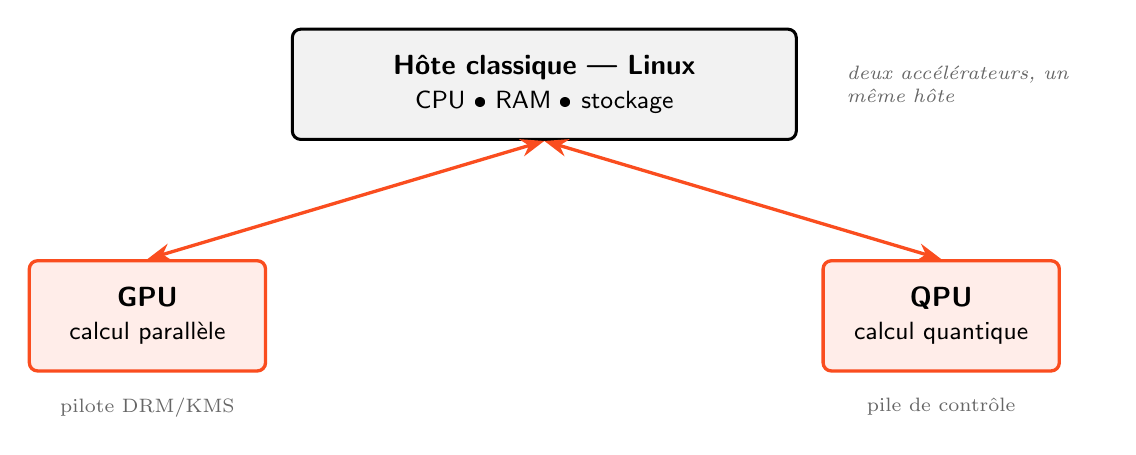
\begin{tikzpicture}[font=\sffamily,
  host/.style={draw=NouBlack,line width=1.1pt,rounded corners=3pt,align=center,minimum width=6.4cm,minimum height=1.4cm,fill=black!5},
  acc/.style={draw=NouOrange,line width=1.2pt,rounded corners=3pt,align=center,minimum width=3cm,minimum height=1.4cm,fill=NouOrange!10}]
  \node[host] (h) {\textbf{Hôte classique — Linux}\\{\small CPU \textbullet{} RAM \textbullet{} stockage}};
  \node[acc,below left=1.5cm and 0.3cm of h] (gpu) {\textbf{GPU}\\{\small calcul parallèle}};
  \node[acc,below right=1.5cm and 0.3cm of h] (qpu) {\textbf{QPU}\\{\small calcul quantique}};
  \draw[{Stealth[length=3mm]}-{Stealth[length=3mm]},NouOrange,line width=1.2pt] (h.south) -- (gpu.north);
  \draw[{Stealth[length=3mm]}-{Stealth[length=3mm]},NouOrange,line width=1.2pt] (h.south) -- (qpu.north);
  \node[below=0.2cm of gpu,font=\scriptsize,NouBlack!60,align=center]{pilote DRM/KMS};
  \node[below=0.2cm of qpu,font=\scriptsize,NouBlack!60,align=center]{pile de contrôle};
  \node[right=0.5cm of h,font=\scriptsize\itshape,NouBlack!60,align=left,text width=3.2cm]{deux accélérateurs, un même hôte};
\end{tikzpicture}
\end{document}
